\documentclass{article}
\usepackage[utf8]{inputenc}

\usepackage{hyperref}
\usepackage{amsmath}
\usepackage{graphicx}

\usepackage{biblatex}
\addbibresource{biblio.bib}

\title{Advanced Learning Models:\\ Kaggle data challenge\footnote{\url{https://www.kaggle.com/c/advanced-learning-models}}}
\author{Ondřej Borovec}
\date{February 2018}

\begin{document}

\maketitle

\section{Introduction}

The main goal of that data challenge, which is part of the Advance learning models course (Ensimag), is to implement and evaluate an learning algorithm on structured data. In this case it is about predicting whether a DNA sequence region is binding site to a specific transcription factor.  

Transcription factors (TFs) are regulatory proteins that bind specific sequence motifs in the genome to activate or repress transcription of target genes. Genome-wide protein-DNA binding maps can be profiled using some experimental techniques and thus all genomics can be classified into two classes for a TF of interest: bound or unbound. In this challenge, we will work with three datasets corresponding to three different TFs.

For this work, no machine learning libraries are allowed.

\section{State of the art}

Binary classification is well known and studied problem of machine learning, where the decision is made based on a feature space. The problem is, sequences do not have explicit features and is not easy to transport sequence into standard feature representation without losing its sequential feature. Then even with very sophisticated feature extraction the dimension of such feature space may not be manageable by standard machines.

There are 3 main approaches for sequence classification in \cite{xing2010brief}: feature based, sequence distance and model based. In this work we decided to work the first one mentioned. Since simple bag-of-words is never sufficient, \cite{xing2010brief} proposes k-gram feature extraction to capture more properties. Such features are from class of permutations with repetition, it means that the size growths exponentially with the size of k-grams. According to this paper, using k-gram features is then suitable for most of the conventional classification methods as Bayes classification, decision trees or SVM. 

DNA sequences along with time series are the main objects of sequence classification problem. \cite{cao2014protein} proposes additionally to k-grams hashing and feature extraction based on the 6-letter exchange group to reduce potential high dimensional feature space. The basic ELM and the OP-ELM, are adopted for the ensemble based SLFNs with slightly better results than SVM.


Currently, the convolution Neural networks(CNN) seems to be the best choice according to \cite{zeng2016convolutional}. Unfortunately, the paper does not give any quantitative comparison to the traditional machine learning classifiers. 


\section{Implementation}

For the purpose to estimate the best practise for working this this dataset we split the training dataset no.1 in to private training and testing part (90\%:10\%). And the first task was to transport sequences into k-grams/features. It can be said, that, generally speaking, more features is beneficial to classifiers, but as was discussed earlier, with increasing size of k-grams, the feature space growths exponentially. It negatively effects learning time, but also size of required memory, which is even more constraining than the time consumption. From my experience this 2000 samples we have not able to create a feature space bigger than for 8-grams. 

We did not implement any feature selection algorithm as PCA of any of the proposed in \cite{xing2010brief}, but sparse k-gram creation approach was implemented to decrease the feature space size. Time necessary to create both of the representations is roughly the same, but the memory requirements are diametrically different. In this case, the full representation of k-grams up to size 8 was not able to fit into memory of our machine, but after implemeting the sparse approach we had not problem with up to the 15-grams.

Another important segment is used model. In general it is true, more complex classifying models takes much longer to fit and also to implement. And since we did not find any prove that a more complex model would give much better results, so it is reasonable for the purpose of this challenge to start with implementation of a standard approach.

The final used model has to be implemented without using any machine learning library, but for the research reason we used python sklearn to test, which standard model would be the best to use. In figure \ref{fig:standard_models_coparison} some standard classifying models with their default params are compared from the point of view of accuracy over the maximum k-grams used for feature matrix creation.

\begin{figure}[h]
    \centering
    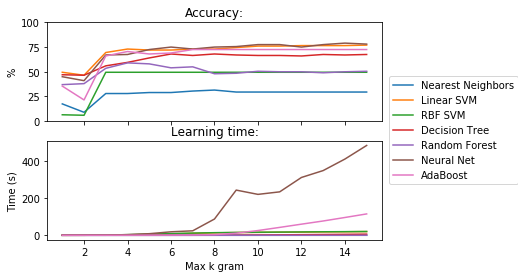
\includegraphics[width=1\textwidth]{imgs/limitedSparseKgramsAccuracyTime.png}
    \caption{Accuracy comparison of standard sklearn model for classification over maximum used k-grams.}
    \label{fig:standard_models_coparison}
\end{figure}

As was expected from the previous research, the leading belongs to Linear SVM and Neural nets wit accuracy of their default implementation around 75\%. Another important observation is that accuracy does not increase linearly with the maximum used k-grams. There is a big jump for 3-grams, but then the increase in not so significant and we can also see a slight decreasing tendencies from time to time. 

The biggest surprise were the bad results of Nearest Neighbors model, but it is a prove that sequence distance based classifiers are more complex then feature based. Then there was also naive Bayes classifier with very good results, but the sklearn implementation does not support sparse matrices, so we dropped it.

Based on the ration between complexity of a model and its accuracy, we decided to implement Linear SVM for the purpose of this data challenge. It mean we are optimizing following equation with Hinge error and L2 normalization:

\begin{equation}\label{eq:svm}
\frac{1}{n}\Big(\sum_{(x, y) \in X} max(0, 1 - y (w * x + b))\Big) + \lambda \| w \|^2
\end{equation}

, where $X$ is set of all samples and $\lambda$ is regularization parameter. For this minimization gradient descent is used with this update rules:


\begin{equation}\label{eq:svm_update}
\begin{split}
w^{i+1} & = w^i -  \frac{1}{|S'|} \Big(\sum_{(x, y) \in X'} -y * x\Big) - \lambda * 2 * w\\
b^{i+1} & = b^i + sign\Big(\sum_{(x, y) \in X'} y\Big)
\end{split}
\end{equation}

Based on the results in figure \ref{fig:standard_models_coparison} we can say, we are going to used 10-grams since higher level, do not help much. Then there is just one hyper parameter of out model - regularization parameter. Since the dimension of our feature vector is much higher than number of samples, we had to implement cross validation for find the best regularization parameter for that data.

As can be seen in figure \ref{fig:reg_param_coparison}, effect of regularization weight on SVM model is not smooth, but we got the best results for $\lambda ~ 0.205$, which we use as the hyper parameter for the final implementation.

\begin{figure}[h]
    \centering
    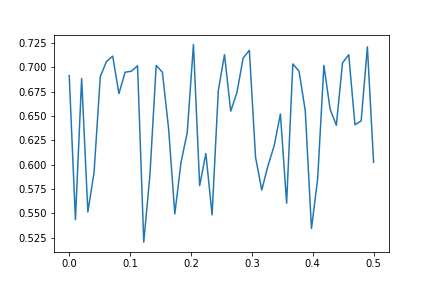
\includegraphics[width=1\textwidth]{imgs/reg_weight_accuracy.png}
    \caption{Accuracy of SVM model for different values of regularization weight.}
    \label{fig:reg_param_coparison}
\end{figure}

\section{Conclusion}

With in this project, we studies the state of the art of Sequence classification and used standard classification models of sklearn to illustrate the possibilities. We also had to find the best representation to capture the data features using sparse feature space representation. As the main part, SVM classifier was implemented using gradient decent optimization along with cross validation to estime the best hyper parameter of that model.

All the code and reseach sheets are attached and also can be found in this github repository\footnote{\url{https://github.com/OBorovec/Ensimag_AML}}

\printbibliography
\end{document}
